\documentclass{article}

%%%%%%%%%%%%%%%%%
%
% Packages here
%
%%%%%%%%%%%%%%%%%
\usepackage[a4paper, margin=1in]{geometry}
\usepackage[utf8]{inputenc}
\usepackage{graphicx}
\usepackage{ctex}
\usepackage{amsmath}
\usepackage{multicol}
\usepackage{tcolorbox}
\usepackage{fontspec}
\usepackage[colorlinks=true, linkcolor=blue]{hyperref}
\usepackage{graphicx}
\usepackage{longtable}

%%%%%%%%%%%%%%%%%%%
%
% Fonts here
%
%%%%%%%%%%%%%%%%%%%

\setCJKmainfont{simsun.ttc}[Path=fonts/, BoldFont=simhei.ttf, ItalicFont=simkai.ttf]
\setCJKmonofont{simfang.ttf}[Path=fonts/]


%%%%%%%%%%%%%%%%%%%%
%
% Title here
%
%%%%%%%%%%%%%%%%%%%%
\title{公务员考试行测复习资料}
\author{IViDerNvI}
\date{\today}


%%%%%%%%%%%%%%%%%%%%
%
% Document here
%
%%%%%%%%%%%%%%%%%%%%
\begin{document}

\maketitle
\newpage
\tableofcontents
\newpage

\section{资料分析}

\subsection{基本公式及导出公式}

\subsubsection{基本公式}

定义 B 为期末额,A 为期初额,r 为增长率,则有以下基本公式:

\begin{equation*}
	\begin{cases}
		r = \frac{B-A}{A} \\
		B = A(1+r)        \\
		A = \frac{B}{1+r} \\
	\end{cases}
\end{equation*}

\subsubsection{导出公式}
\paragraph{隔期增长率}
定义 B 为期末额,A 为期初额,$r_1,r_2$ 分别为期初-期中增长率和期中-期末增长率,则有总增长率$r$:
\[
	r = r_1 + r_2 + r_1r_2
\]

\paragraph{部分增长率}

将总额分成两部分,定义$B_1$ 为分1期末额,$A_1$ 为分1期初额,$r_1$ 为分1增长率,$B_2$ 为分2期末额,$A_2$ 为分2期初额,$r_2$ 分2增长率,$B$ 为总期末额,$A$ 为总期初额,$r$ 为总增长率。则有:

\[
	r = \frac{A_1}{A}r_1 + \frac{A_2}{A}r_2
\]

\paragraph{乘积增长率}

定义 $B_1,B_2$ 为期末额,$A_1,A_2$ 为期初额,$r_1,r_2$ 为增长率,则两个量的乘积的增长率为:

\[
	r = r_1 + r_2 + r_1r_2
\]

\paragraph{比值增长率}

定义 $B_1,B_2$ 为期末额,$A_1,A_2$ 为期初额,$r_1,r_2$ 为增长率,则两个量的比值的增长率为:

\[
	r = \frac{r_1-r_2}{1+r_2}
\]

\paragraph{期初比重和期末比重}

将总额分成两部分,定义$B_1$ 为分1期末额,$A_1$ 为分1期初额,$r_1$ 为分1增长率,$B$ 为总期末额,$A$ 为总期初额,$r$为总增长率(即从$\frac{A_1}{A}$增长到$\frac{B_1}{B}$)。则:
\[
	\frac{A_1}{A} \frac{1+r_1}{1+r} = \frac{B_1}{B}
\]

\paragraph{比重增长率}

将总额分成两部分,定义$B_1$ 为分1期末额,$A_1$ 为分1期初额,$r_1$ 为分1增长率,$B$ 为总期末额,$A$ 为总期初额,$r$为总增长率(即从$\frac{A_1}{A}$增长到$\frac{B_1}{B}$)。则部分占比的增长率为:
\[
	r^\prime = \frac{r_1-r}{1+r}
\]

\paragraph{比重差}
将总额分成两部分,定义$B_1$ 为分1期末额,$A_1$ 为分1期初额,$r_1$ 为分1增长率,$B$ 为总期末额,$A$ 为总期初额,$r$为总增长率(即从$\frac{A_1}{A}$增长到$\frac{B_1}{B}$)。则比重差为:
\[
	\frac{B_1}{B} - \frac{A_1}{A} = \frac{r_1 - r}{1+r}\frac{A_1}{A} = \frac{A_1}{B} (r_1-r)
\]

\subsection{计算方法}

\subsubsection{小分互换法}

\paragraph{使用场景} 某个大数除以一个整数,可以转化为一个大数乘以一个百分数.

\paragraph{案例} 例如: 求 $235 \div 7$, 就可以转化为 $235 \times 0.142857$, 可以初步计算为$23.5 + 9.2 + 0.46 \approx 33.16$

\paragraph{常见小分互换} 一些常见的小分互换可以帮助快速计算:

\begin{multicols}{2}
	\begin{enumerate}
		\item $\frac{1}{2} = 0.500$
		\item $\frac{1}{3} = 0.330$
		\item $\frac{1}{4} = 0.250$
		\item $\frac{1}{5} = 0.200$
		\item $\frac{1}{6} = 0.167$
		\item $\frac{1}{7} = 0.143$
		\item $\frac{1}{8} = 0.125$
		\item $\frac{1}{9} = 0.111$
		\item $\frac{1}{10} = 0.100$
		\item $\frac{1}{11} = 0.091$
		\item $\frac{1}{12} = 0.083$
		\item $\frac{1}{13} = 0.077$
		\item $\frac{1}{14} = 0.071$
		\item $\frac{1}{15} = 0.067$
		\item $\frac{1}{16} = 0.063$
		\item $\frac{1}{17} = 0.059$
		\item $\frac{1}{18} = 0.056$
		\item $\frac{1}{19} = 0.053$
	\end{enumerate}
\end{multicols}

\subsubsection{拆分法}

\paragraph{使用场景} 当一个数乘以一个百分数时, 将这个百分数凑到最近的便于计算的数字.

\paragraph{案例} 例如: 求 $235 \times 0.14$, 就可以转化为 $235 \times (0.1 + 0.04)$, 可以初步计算为$23.5 + 9.4 \approx 32.9$

\paragraph{常见拆分} 一些常见的拆分可以帮助快速计算:

\begin{multicols}{2}
	\begin{enumerate}
		\item $45\% = 50\% - 5\%$
		\item $55\% = 50\% + 5\%$
		\item $15\% = 10\% + 5\%$
		\item $60\% = 50\% + 10\%$
		\item $95\% = 1 - 5\%$
		\item $90\% = 1 - 10\%$
	\end{enumerate}
\end{multicols}


\newpage
\section{逻辑推理}

\subsection{逻辑部分}

\subsection{类比推理}

\subsubsection{类比推理的基本关系}

\paragraph{全同关系} 二者是同一事物的不同称呼

\paragraph{包含关系} 包括组成关系和种属关系

\paragraph{并列关系} 二者是同类事物的不同内容,包括结构并列和含义并列

\paragraph{交叉关系} 二者是不同的分类方式,互有重叠

\paragraph{对立关系} 包括矛盾关系和反对关系(矛盾指两者完全互斥,非此即彼;反对指两者不相交,但并不一定互斥)

\paragraph{前后关系} 二者是事物发展的先后顺序

\paragraph{联系关系} 近年来的高频考点,主要包括:

\begin{itemize}
    \item 功能联系:包括主要功能和次要功能
    \item 原材料联系:事物的原材料或者材质
    \item 场所联系:作用的场所或发生的地点
    \item 时间联系:包括先后顺序等(尤其考虑时间联系的紧密程度,十二时辰中各个时辰间隔程度)
    \item 因果联系:二者是事物运动的因果联系
    \item 职业联系:二者是职业或行业的联系
\end{itemize}

\subsubsection{类比推理的常见考法}

见附录\ref{trd:appendix}。



\newpage

\subsection{图推部分}
\newpage
\section{言语理解}

\subsection{一般性原则}

\paragraph{主体一致性原则}

主体一致原则是指, 文段和选项所讲述的主体要一致。比如文段讲的是“三农问题”,选项讲的是“智慧农业”,则不符合主体一致性原则。通常情况下, 主体会在文段中反复提及, 也会在总结句中首次表达, 需要厘清其中关系。

\begin{quote}
	\textbf{一定要注意文段''主要讲述''和''举例子''的区别:}
	\begin{tcolorbox}[colback=blue!5, colframe=blue!75!black, title=主体一致性案例1]
		\textit{原始体育的萌芽与日复一日地生产劳动分不开,跳绳运动也不例外。古时,跳绳所用的绳被称为“绳索”,它是由古人编结而成的,人们在编绳索的过程中,通常会有一些跨越的动作,这些下意识的行为吸引了活泼好动的孩子,他们就用短的绳子在旁边反复模仿,并逐渐摸索出一些简单的跨越绳子的方法,当成一种游戏来玩,于是跳绳这一活动就产生了。对于跳绳的明确起源众说纷纭。最早出现的史料是汉代画像石上的跳绳图,证明当时已有了跳绳活动。南朝《荆楚岁时记》中有“飞百索”的记载,正是后来的跳绳游戏。}
		\tcblower%ww
		\texttt{此段文章只在开头提到原始体育, 作为背景资料, 引出跳绳运动也与劳动分不开。文章主体是跳绳运动, 所以以“原始体育”为主体的不符合主体一致性原则。}
	\end{tcolorbox}
\end{quote}

\begin{quote}
	\textbf{内容相近一定要注意文段主体:}
	\begin{tcolorbox}[colback=blue!5, colframe=blue!75!black, title=主体一致原则案例2]
		\textit{成绩要求相对较低,导致部分考生视艺考为进入高等学府的“绿色通道”或迅速成名的捷径,于是扎堆报考、突击报考等现象也就随之出现。另外,由于高中教学与艺考不能有效衔接,一个巨大的艺考培训市场应运而生,但市场内部存在行业垄断、恶性竞争、干扰院校招考正常秩序等乱象,破坏了艺术类专业招生和培养的健康生态。对此,教育部门应针对时弊,对艺术类专业招生加强规范,严格入校管理,进一步完善优化招录程序。}\\
		这段文字意在说明:\\
		A.“艺考”不等于“易考”\\
		B.艺术类专业招生亟待规范\\
		C.艺术类人才更需提升文化素养\\
		D.教育部门应多举措促进艺考公平
		\tcblower%ww
		\texttt{关注 B, D 选项, 两者都提到规范作用,但是看到文段中强调主体为'艺术类专业招生', 故选择 B 选项}
	\end{tcolorbox}
\end{quote}

\paragraph{对策优先原则}

对策优先原则是指, 文段中如果有对策类的内容, 则选项中也要有对策类的内容。比如文段中提到“我们应该采取措施来解决问题”,则选项中也要有“我们应该采取措施”这样的表述。

\begin{quote}
	\textbf{文段只描述问题时也可以酌情选择对策:}
	\begin{tcolorbox}[colback=blue!5, colframe=blue!75!black, title=对策优先原则案例]
		\textit{人车争道是影响我国城市交通安全的顽疾之一。“斑马线之争”不仅让市民出行心惊胆战,造成交通拥堵事故频发,还严重影响了公共交通文明和城市形象。据公安部交管局统计,近三年来,全国共在斑马线发生机动车与行人的交通事故 1.4 万起,造成 3898 人死亡。}\\
		这段文字主要阐述的是:\\
		A.交通出行与每个人生活息息相关\\
		B.倡导礼让斑马线需要长期坚持\\
		C.斑马线文明是城市文明的缩影\\
		D.机动车驾驶员法律意识、文明意识淡薄
		\tcblower%
		\texttt{文段表述了交通问题的严重, 没有给出解决方案, 选项 B 中的'倡导礼让斑马线'看作对策是针对题中`斑马线问题`的回答, 故选择 B 选项}
	\end{tcolorbox}
\end{quote}


\subsection{文段分类}

\subsubsection{文段类型分类}

\paragraph{说理文}

说理文是以说理为主要目的的文章,通常存在着号召、劝说、启发、警示等目的。在选择主旨大意时\textbf{优先选择阐明道理}的选项。

\paragraph{科普文}

科普文是以传播科学知识为主要目的的文章,通常存在着介绍、说明、分析等目的。在选择主旨大意时\textbf{优先选择介绍事物原理}的选项。

\paragraph{新闻文}

新闻文是以传播新鲜事物为主要目的的文章,通常存在着介绍、报道、评论等目的。在选择主旨大意时\textbf{优先选择表述新突破新进展}的选项。

\subsubsection{文段对策分类}

\paragraph{祈使建议}

文段中包含''应该''、''必须''、''要求''、''可以''、''建议''等词语时, 应当优先选择''建议''、''对策''、''措施''等选项。

\paragraph{禁止否定}

文段中包含''不允许''、''禁止''、''不可以''、''避免''等词语时, 应当优先选择''禁止''、''否定''等选项。

\paragraph{逻辑关联}

文段中包含''如果$\dots$才''、''只有$\dots$就''、''必须$\dots$否则''等词语时, 应当优先选择''因果关系''、''条件关系''等选项。

\paragraph{必要条件}

文段中包含``必须``、``必要``、``不可或缺``等词语时, 应当优先选择``必要条件``、``前提条件``等选项。

\paragraph{语义强调}

文段中包含''时代命题''、''必经之路''等词语时, 应当优先选择''强调''、''特别注意''等选项。

\subsubsection{文段结构分类}
\paragraph{总分结构} 总分结构优先选总结句, 其次是所有分论点的概括
\begin{multicols}{2}
	\begin{enumerate}
		\item 此外 + 分
		\item 这些 + 总
	\end{enumerate}
\end{multicols}

\paragraph{并列结构} 答案要涵盖文段并列的所有内容
\paragraph{转折结构} 转折结构优先选择转折前+后的内容, 其次是转折前后的内容
\paragraph{对比结构} 对比结构优先选择对比前+后的内容, 其次是对比前后的内容
\paragraph{因果结构} 因果结构优先选择 xxx 的原因选项
\paragraph{背景+内容} 背景+内容优先选择同内容表述一致的选项

\begin{quote}
	\textbf{背景知识也需要考虑}
	\begin{tcolorbox}[colback=blue!5, colframe=blue!75!black, title=背景+内容案例]
		\textit{传统的文明标准有三个,即文字、青铜器和城市。但后来许多考古学家发现,由于区域不同,文明的
			差异也很大,这个判断标准不但行不通,还会给考古工作带来阻碍。现如今,国际上对文明的判断标准主
			要是:已进入国家社会形态,具有一套礼仪系统和统治管理制度。良渚文化虽未有青铜器和较为成熟的文
			字,但具有早期国家社会形态和较为完整的礼仪系统以及管理制度,还具有许多东方文明的因素。有良渚
			文化考古研究员甚至认为,良渚文化是东方早期一个集大成的文明。}
		\tcblower%ww
		只看内容部分`\textit{虽未有青铜器和较为成熟的文字,但具有早期国家社会形态}`可以得出答案应该表述为 xx 颠覆了通常标准的选项. 但是要看到背景处`\textit{已进入国家社会形态,具有一套礼仪系统和统治管理制度}`的表述则需要选择满足通行文明判断标准的选项
	\end{tcolorbox}
\end{quote}

\paragraph{设问+内容} 设问+内容优先选择同回答设问的内容表述一致的选项


\subsection{题干分类}

\subsubsection{下面讲述}

\paragraph{文段讲述问题} 下文讲述解决问题的方法或者问题出现的原因
\begin{quote}
	\textbf{解决问题和分析问题同时出现时优先分析问题}
	\begin{tcolorbox}[colback=blue!5, colframe=blue!75!black, title=文段讲述问题案例]
		\textit{冬季是心血管疾病的高发季节。相关研究数据表明,每年的 12 月至次年 3 月是心血管病发病高峰期,发病数明显高于其他月份,这与血脂季节性波动的结论也相一致。据统计数据显示,因心血管疾病死亡事件中约 15.8\%与天气寒冷相关,而仅有 1.3\%与天气炎热相关。心力衰竭、心肌梗死和脑卒中在寒冷季节的发病率和死亡率均高于温暖季节。}\\
		这段文字接下来最有可能讲的是:\\
		A.心血管疾病为何冬季高发\\
		B.心血管疾病的症状有哪些\\
		C.如何有效治疗心血管疾病\\
		D.如何预防冬季心血管疾病
		\tcblower%
		\texttt{A,D分别讲的是文段提出问题的分析和解决方式,同时出现时优先选择问题分析,故选A}
	\end{tcolorbox}
\end{quote}

\paragraph{文段提出新概念} 下文解释新概念
\paragraph{文段给出总对策} 下文具体展开内容
\paragraph{文段提出过去内容} 下文讲述当今的新特点
\begin{quote}
	\begin{tcolorbox}[colback=blue!5, colframe=blue!75!black, title=文段提出过去内容案例]
		\textit{以往我们的农民形象塑造形成两种习惯性模式:一种是正面讲述主人公如何在改革与保守或先进与落后等二元对立中凭借忍辱负重、自我牺牲或善良人品等方式化敌为友,赢得村民信赖,取得改革的进展;另一种则是通过主人公的一连串小品化或喜剧化故事去消解矛盾,保持对观众的吸引力。这两种习惯性模式的美学后果在于,农民形象几乎成了一成不变的符号,缺乏应有的丰富性和吸引力,与现实生活存在巨大落差。这种模式是对真实本身的扁平化。}\\
		这段文字接下来最可能说的是:\\
		C.现在塑造的农民形象有什么改变
		\tcblower%
		\texttt{注意首句'以往',末尾提到两个模式的问题,故下文应强调现在的变化}
	\end{tcolorbox}
\end{quote}

\subsubsection{最佳题目}

\paragraph{措施优先原则}

文段若是说理文、则选号召的措施

\paragraph{新闻选新原则}

文段若是新闻稿,则优先选择新闻的''新''

\subsubsection{填入语句}

\paragraph{填入语句在开头} 填入语句可能是总概括、引出话题(包含主题词)、转折引出观点或对策等。(国考用俗语引出概率较大)
\paragraph{填入语句在中间} 填入语句可能是承上启下、前对策(后文是论证)、提出问题(后文是对策)等。
\paragraph{填入语句在结尾} 填入语句多为总结或对策句,注意首尾呼应。
\paragraph{其他注意} 填入语句要和前后句关系正确,要注意语法结构正确(主谓宾搭配得当)、逻辑关联词运用得当、全
文主语一致、后文指示代词指代正确;可特别考虑句式一致。

\begin{quote}
	\begin{tcolorbox}[colback=blue!5, colframe=blue!75!black, title=考虑句式一致]
		\textit{讲好中国故事、传播好中国声音,习近平总书记为我们树立了光辉典范。引用当地谚语、结合个人经历、 讲述感人故事……党的十八大以来, 习近平总书记在出访、 出席重要国际会议、 会见来访外国客人时,用外界听得懂的语言,\underline{\hspace{2cm}}。}\\
		填入文中画横线部分最恰当的一项是:\\
		A.创新对外话语表达,展示真实、立体、全面的中国\\
		B.以润物细无声的方式,增进世界对中国的了解\\
		C.立足本国,面向世界,让中国文化不断传播出去\\
		D.让中国理念、中国主张、中国方案更具触发共鸣的力量\\
		\tcblower%
		\texttt{B选项中'以润物细无声的方式'与'用外界听得懂的语言'对仗,优先选择}
	\end{tcolorbox}
\end{quote}

\subsubsection{语句排序}

\paragraph{整体把握} 把握结构特点(总分、并列)
\paragraph{细节把握} 下定义是首句的概率较大,指代一定要有前文
\paragraph{逻辑关系} 因果、转折、递进等关系确定两个一定相邻的子句

\subsubsection{细节判断}

\paragraph{细节题错误设置} 偷换概念,混淆时态,杂糅,本身有误(和实际不符),绝对化,无中生有


\subsection{选项分类}

\subsubsection{错误分类}

\paragraph{出处错误} 背景、例子、分析论证中提炼的选项出处有误,一般不选
\paragraph{片面}原文并列谈论两方面,只说一方面的不能选(选项为对策可包容此问题)
\paragraph{杂糅}选项为原文中各个句子中提炼词语拼凑而成
\paragraph{绝对化}最高级、必要条件,原文未提及时不能选
\paragraph{下定义}即中性表达,介绍说明,在说理类文段题目中不选
\paragraph{无中生有}选项中的关键信息原文未提及
\paragraph{本身有误}即选项本身不符合事实,逻辑错误或不符合主流价值观等

\subsubsection{表述分类}

\paragraph{原因类}
文段为因果或果因结构,或整个文段是“选项”的原因;
\begin{quote}
	\begin{tcolorbox}[colback=blue!5, colframe=blue!75!black, title=原因类选项案例]
		\textit{员工家庭福利政策的长期缺失,虽然给企业带来了成本降低、产量提高等显而易见的优势,但对员工而言,抛弃年幼的孩子和年迈的父母,显然不是合理的职业规划。一些经济学家认为,家庭福利政策的匮乏实际上反映了美国经济中企业和员工之间权利不平衡的状态。经济产出流入公司利润的份额在飙升,而员工的薪酬却停滞不前,这必然会导致美国陷入人才流失的困境。}\\
		C. 揭示美国人才流失的深层次原因
		\tcblower%
		\texttt{文章中提到'这必然会导致美国陷入人才流失的困境', 但这里并不能够选择原因类选项, 因为其本身并非已经引发的社会现象, 于是无法归因}
	\end{tcolorbox}
\end{quote}

\paragraph{历程类} 文段一般有清晰时间轴,介绍整个发展历程

\paragraph{具体类} 可归纳概括出具体小点 ''12345'' (类似申论概括题目) 或展开介绍其中的''1''

\paragraph{比较类} 文段有双主语,双主语地位相当,论述篇幅也大致相当

\paragraph{宽泛+具体} 选项中宽泛和具体的选项同时出现时选择具体的选项

\begin{quote}
	\begin{tcolorbox}[colback=blue!5, colframe=blue!75!black, title=宽泛+具体案例]
		\textit{教材是用来教育的,什么样的教材决定了孩子们将接受什么样的教育。这是公众关注课改的实质。然而长期以来,在教材编写方面,一直缺乏畅通公众意见的制度管道。这是因为我国实行的是一种编、审、用一体化的集权型体制,教材编写机构编什么,学生就得接受什么,即使是对教材的审定,也仍是一种体内循环机制。这种教材编写模式的结果是,我们只可能有一本教材,学校没有其他选择的可能。显然,在一个有着越来越多公众表达的时代,这种自闭式教材编写模式,没得到重视与警惕。}\\
		这段文字意在表明:\\
		A.教材编写应听取公众意见\\
		B.教材的编写模式亟需改变\\
		C.自闭式教材编写不符合时代发展\\
		D.教材编写直接影响孩子教育
		\tcblower%
		\texttt{选项 B, C 和 D 都是宽泛的表述, 即指出存在的问题而没有点出具体的解决方案, 故指出解决方案的选项 A 正确}
	\end{tcolorbox}
\end{quote}



\newpage
\section{数量关系}

\subsection{方程法}

\subsubsection{不定方程}

\paragraph{倍数与不定方程} 列方程、消元至二元方程,依靠实际意义(取整数)来判断

\begin{quote}
	\textbf{倍数与不定方程}
	\begin{tcolorbox}[colback=red!5!white, colframe=red!75!black, title=倍数与不定方程]
		\textit{某人花 400 元购买了若干盒樱桃。已知甲、乙、丙三个品种的樱桃单价分别为 28 元/盒、32 元/盒和33 元/盒,问他最多购买了多少盒丙品种的樱桃?}\\
		A.3 B.4\\
		C.5 D.6
		\tcblower%
		\texttt{设购买了 $x$ 盒丙品种的樱桃,则有 $33x + 28y + 32z = 400$, 其中 33x 应当为4的倍数,故而选B}
	\end{tcolorbox}
\end{quote}

\subsection{工程问题}

\subsubsection{给定工作时间}

\paragraph{套路} 设工作总量为工作效率的公倍数,求出各部分效率,再求题目所要求数据

\subsubsection{给定效率比}

\paragraph{套路} 效率比作为效率,计算工作总量,再求题目所要求数据

\subsubsection{给定不同完工情况}

\paragraph{套路} 根据工作总量一定列方程

\subsection{合作完工问题}

\subsubsection{合作完工问题的性质}

设 $A, B$ 二人合作完成一项工作,工作总量为 $S$,各自的工作效率分别为 $a, b$,二人分别休息了$x, y$的时间, 且休息时间不重叠, 设总工时为t, 则有:
\[
	t = \frac{S}{a + b} + x + y
\]


\subsection{整除问题}

\subsubsection{整除的性质1}

若不定方程中解出 $y = \frac{a}{b}x, \gcd (a, b) = 0$, 则一定有:
\[
	x = bn, y = am, \forall n, m \in Z
\]

\subsubsection{整除的性质2}

若最后 1 位能被 2 或 5 整除,则该数能被 2 或 5 整除
若最后 2 位能被 4 或 25 整除,则该数能被 4 或 25 整除
若最后 3 位能被 8 或 125 整除,则该数能被 8 或 125 整除

\subsubsection{整除的性质3}

若数字的和能被 3 整除,则该数能被 3 整除
若数字的和能被 9 整除,则该数能被 9 整除


\subsection{余数问题}

\subsubsection{余数的性质}

\paragraph{余同取余} 若 $x$ 除以 $m$ 余 $a$,$y$ 除以 $n$ 余 $a$,则有:

\[
	x = k\gcd (m,n) + a, \forall k \in Z
\]

\paragraph{和同加和} 若 $x$ 除以 $m$ 余 $a$,$y$ 除以 $n$ 余 $b$,且 $a + m = b + n$,则有:

\[
	x = k\gcd (m,n) + a + m, \forall k \in Z
\]

\paragraph{差同减差} 若 $x$ 除以 $m$ 余 $a$,$y$ 除以 $n$ 余 $b$,且 $a - m = b - n$,则有:

\[
	x = k\gcd (m,n) + a - m, \forall k \in Z
\]

\subsection{等差数列}

\subsubsection{等差数列的性质}

\[
	S = n \times a_{mid} = \frac{n}{2} \times (a_1 + a_n)
\]

\subsection{容斥问题}

\subsubsection{容斥原理}

\paragraph{容斥原理} 设 $A, B$ 是有限集合,则有:
\[
	|A \cup B| = |A| + |B| - |A \cap B|
\]

\begin{center}
	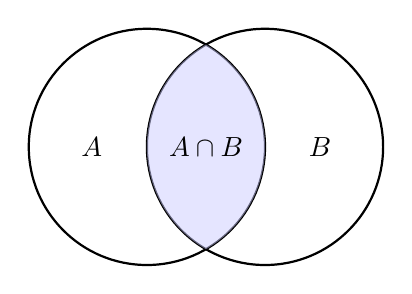
\begin{tikzpicture}
		% Draw circles
		\draw[thick] (0,0) circle (1.5);
		\draw[thick] (1.5,0) circle (1.5);
		% Labels
		\node at (-0.7,0) {$A$};
		\node at (2.2,0) {$B$};
		% Intersection shading
		\begin{scope}
			\clip (0,0) circle (1.5);
			\fill[blue!20, opacity=0.5] (1.5,0) circle (1.5);
		\end{scope}
		% Intersection label
		\node at (0.75,0) {$A \cap B$};
	\end{tikzpicture}
\end{center}

\begin{center}
	\textbf{图\thesubsubsection-\thefigure:集合 $A$ 与 $B$ 的并集与交集示意图}
\end{center}

\subsection{平方数}

\subsubsection{常见平方数}

\begin{multicols}{2}
	\begin{enumerate}
		\item $11^2 = 121$
		\item $12^2 = 144$
		\item $13^2 = 169$
		\item $14^2 = 196$
		\item $15^2 = 225$
		\item $16^2 = 256$
		\item $17^2 = 289$
		\item $18^2 = 324$
		\item $19^2 = 361$
	\end{enumerate}
\end{multicols}

\subsection{溶质与溶液}

\paragraph{基本思路} 设溶液浓度为 $r_i$, 溶液质量为 $A_i$, 混合溶液浓度为 $r$, 则:
\[
	\sum_{i}A_i r_i = r\sum_{i}A_i
\]

\subsubsection{基本题型}

\paragraph{题型一} 溶液加两次水. 溶液蒸发后加水. 溶液加水后蒸发.

\paragraph{题型二} 高低浓度溶液混合. 使用十字交叉法, 整体法.

\subsection{经济利润问题}

\subsubsection{基本概念}

\paragraph{模型} 经济利润 = 收入 $-$ 成本

\subsubsection{解法}

\paragraph{方程法}
\newpage
\section{常识判断}

\subsection{法律知识}

\subsubsection{国家的基本制度}

\paragraph{人民民主专政制度} 人民民主专政是我国的国体,其主要特色有中国共产党领导的多党合作和政治协商制度、爱国统一战线。

\paragraph{人民代表大会制度} 我国政权的组织形式,政体,根本政治制度,其基本内容为:

\begin{itemize}
	\item 国家的一切权利属于人民
	\item 人民在民主基础上选派代表,组成全国人大和地方人大作为权力机关
	\item 国家检察机关、监察机关、审判机关、行政机关由人大产生,对它负责,受它监督
	\item 人民代表大会常务委员会对本级人民代表大会负责,人民代表大会对人民负责
\end{itemize}

\paragraph{基本经济制度} 在社会主义初级阶段,坚持公有制为主体、多种所有制经济共同发展,坚持按劳分配为主体、多种分配方式并存。国家实行社会主义市场经济。社会主义公有制是我国经济制度的基础,非公有制经济是社会主义市场经济的重要组成部分。

\paragraph{选举制度} 其原则包括普遍性原则,平等原则,直接选举和间接选举并用原则,秘密投票原则。

\paragraph{特别行政区制度} 特别行政区享有高度自治权,包括行政管理权,立法权,独立的司法权和终审权,自行处理有关对外事务的权力。除外交和国防事务外,中央政府不干预特别行政区的内部事务。全国人大具有备案审查权,特别行政区制定的基本法须在全国人大备案,备案不影响其生效,全国人大可发回其中条款,发回的条款除另有规定外,立即失效且无溯及力。

\paragraph{民族区域自治制度} 在国家统一领导下,各少数民族聚居的地方实行区域自治,设立自治机关,行使自治权的制度。

\paragraph{基层群众自治制度} 以中国共产党基层组织为领导,依托基层群众自治组织(例如村委会、居委会),在城乡地区实现居民直接行使相关政治权利及所在居民的自我管理、自我服务、自我教育、自我监督的制度。

\subsubsection{公民的基本权利和义务}

\paragraph{公民的基本权利} 公民的基本权利包括平等权,政治权利和自由,监督权和获得赔偿权,宗教信仰自由,社会经济权利,文化教育权利,特定人的权利

\paragraph{公民的基本义务} 服兵役,纳税等

\subsubsection{国家机构}

\paragraph{国家机构的组织和活动原则}

\subparagraph{民主集中制} 民主基础上的集中和集中指导下的民主相结合

\subparagraph{社会主义法制原则} 国家机关和工作人员行使权力必须在法律框架内

\subparagraph{责任制原则} 国家机关和工作人员必须对其行使权力的后果负责

\subparagraph{为人民服务原则} 国家机关和工作人员接受人民监督, 为人民服务

\subparagraph{精简和效率原则} 提高工作效率, 反对官僚主义

\paragraph{全国人民代表大会} 全国人民代表大会是最高国家权力机关,地方各级人民代表大会是地方国家权力机关。

\paragraph{全国人民代表大会常务委员会} 全国人民代表大会常务委员会是全国人民代表大会的常设机关,行使全国人大闭会期间的部分职权。

\paragraph{国家主席} 中华人民共和国主席(简称“国家主席”),是中华人民共和国的国家代表,也是国家机构之一。中华人民共和国主席、副主席由全国人民代表大会选举产生,每届任期同全国人民代表大会每届任期相同。

\paragraph{国务院} 中央人民政府,是最高国家权力机关的执行机关,是最高国家行政机关。国务院由总理、副总理、国务委员、各部部长、各委员会主任、中国人民银行行长、审计长、秘书长组成。国务院实行总理负责制。总理领导国务院的工作。 [1]

\paragraph{中央军事委员会} 直接领导全国武装力量。其组成人员由中国共产党中央委员会决定。

\paragraph{监察委员会} 行使国家监察职能的专责机关,对所有行使公权力的公职人员进行监察,调查职务违法和职务犯罪,开展廉政建设和反腐败工作,维护宪法和法律的尊严。


\newpage
\appendix
\section{附录:成语释义}
\label{fst:appendix}

\begin{longtable}{|p{0.1\textwidth}|p{0.35\textwidth}|p{0.1\textwidth}|p{0.35\textwidth}|}
    \hline
    \textbf{成语} & \textbf{释义}                        & \textbf{成语} & \textbf{释义}               \\
    \hline
    英勇无畏        & 英勇无畏                               & 前仆后继        & 前人倒下了, 后人继续前进             \\
    \hline
    视死如归        & 视死如归, 不怕牺牲                         & 大义凛然        & 正义的样子                     \\
    \hline
    挺身而出        & 勇敢地站出来                             & 勇往直前        & 勇敢地向前走                    \\
    \hline
    踔厉奋发        & 振奋精神, 努力向前                         & 笃行不怠        & 坚定地实践, 不懈怠                \\
    \hline
    赓续前行        & 继续前进                               & 奋楫争先        & 争先恐后, 努力向前                \\
    \hline
    砥砺前行        & 克服困难, 坚持前进                         & 勇毅前行        & 勇敢坚定地向前                   \\
    \hline
    一鼓作气        & 一口气完成, 不松懈                         &             &                           \\
    \hline
    偏听偏信        & 只听一方                               & 亦步亦趋        & 强调跟着别人做                   \\
    \hline
    人云亦云        & 强调跟着别人说                            & 盲从盲信        & 强调不加自考听别人                 \\
    \hline
    玉树临风        & 形容男子英俊潇洒                           & 国色天香        & 形容女子美丽动人                  \\
    \hline
    面如冠玉        & 形容男子面容清秀                           & 螓首峨眉        & 形容女子眉清目秀                  \\
    \hline
    倾国倾城        & 形容女子美丽动人                           & 明眸皓齿        & 形容女性眼眸明亮                  \\
    \hline
    潜移默化        & 环境中受到影响                            & 耳濡目染        & 听看中受到影响                   \\
    \hline
    如沐春风        & 强调打造好环境                            & 润物无声        & 文化教育                      \\
    \hline
    成风化人        & 形成一种风气感化人                          & 耳提面命        & 严格教导                      \\
    \hline
    循循善诱        & 苦口婆心劝导                             & 诲人不倦        & 教育不知疲倦                    \\
    \hline
    春风化雨        & 不强迫教育                              & 和风细雨        & 批评劝导                      \\
    \hline
    振聋发聩        & 唤醒麻木的人                             & 醍醐灌顶        & 一下明白                      \\
    \hline
    颠扑不破        & 比喻真理经得起考验                          & 屡试不爽        & 多次尝试(某种方法)都没有差错           \\
    \hline
    慎终追远        & 谨慎地对待父母的去世,追念祖先的德行                 & 光耀门楣        & 使家族或家庭因某人的成就而荣耀显赫         \\
    \hline
    浑水摸鱼        & 借混乱之机谋取私利                          & 趁火打劫        & 在他人危难时趁机图谋利益              \\
    \hline
    矜功伐善        & 夸耀自己的功劳与优点                         & 色厉内荏        & 外表强硬,内心虚弱                 \\
    \hline
    沸反盈天        & 声音喧闹如沸腾的水,响彻天空。形容极度喧嚣混乱            &             &                           \\
    \hline
    司空见惯        & 常见,强调不足为奇                          & 层见叠出        & 常见                        \\
    \hline
    形如槁木        & 瘦的像木头                              & 江心补漏        & 形容来不及补救                   \\
    \hline
    鲁鱼亥豕        & 一字之差,差之千里                          &             &                           \\
    \hline
    千锤百炼        & 原指金属要经过多次锤打才能成材,后比喻人在艰难困苦中不断磨练、成长。 & 精雕细琢        & 原指雕刻细致入微,后引申为做事认真细致、反复打磨。 \\
    \hline
    精益求精        & 已经很好了,还要求更好,形容追求极致、不断完善。           & 蟾宫折桂        & 指在科举应试得中                  \\
    \hline
    瞠乎其后        & 只能落在后面瞪眼看着,形容远远落后于人。               & 分庭抗礼        & 双方实力相当                    \\
    \hline
    等量齐观        & 可量化的事物能够比较,数量相当                    & 相提并论        & 把不同的事物放在一起比较,强调地位上的比较     \\
    \hline
    同日而语        & 同一事物在不同时期的比较                       & 浩若烟海        & 多指代文献,书籍数量众多              \\
    \hline
    洋洋大观        & 美好的事物数量众多                          & 祸起萧墙        & 指祸乱发生在内部或身边的人             \\
    \hline
    洞若观火 & 形容看得非常清楚明白,像看火一样清晰。                & 了如指掌        & 对事物非常熟悉,了解得很清楚。          \\
    \hline
\end{longtable}


\newpage
\section{附录:词语辨析}
\label{sec:appendix}

\subsection{固定搭配表}

\begin{longtable}{|p{0.1\textwidth}|p{0.35\textwidth}|p{0.1\textwidth}|p{0.35\textwidth}|}
    \hline
    \textbf{词语} & \textbf{释义} & \textbf
    {词语}        & \textbf{释义}                  \\
    \hline
    提供依托        & 提供支撑        & 开启篇章    & 夯实产能 \\
    \hline
    凝聚共识        & 打牢基础        & 厚植动能    & 彰显底色 \\
    \hline
    筑牢根基        & 完善制度        & 落实战略    & 筑牢基础 \\
    \hline
    推进突破        & 形成合力        & 健全体系    & 发挥优势 \\
    \hline
    构建机制        & 历史性转变       & 增强意愿    & 破解难题 \\
    \hline
\end{longtable}

\subsection{成语释义表}

\begin{longtable}{|p{0.1\textwidth}|p{0.35\textwidth}|p{0.1\textwidth}|p{0.35\textwidth}|}
    \hline
    \textbf{词语} & \textbf{释义} & \textbf
    {词语}        & \textbf{释义}                         \\
    \hline
    肇始          & 开始,起始       & 发轫      & 新事物或者局面开始出现 \\

    \hline
\end{longtable}
\newpage
\section{附录:逻辑推理常见词语及关系}
\label{trd:appendix}

\begin{longtable}{|p{0.1\textwidth}|p{0.35\textwidth}|p{0.1\textwidth}|p{0.35\textwidth}|}
    \hline
    \textbf{词语} & \textbf{释义}      & \textbf{词语} & \textbf{释义}        \\
    \hline
    墨鱼,乌贼       & 墨鱼和乌贼是同一种动物的不同名称 & 国有企业,集体企业   & 二者从属于内资企业,互相并列     \\
    \hline
    己所不欲,勿施于人   & 推广关系             & 不入虎穴,焉得虎子   & 充分条件关系             \\
    \hline
    不忘初心,方得始终   & 因果关系             & 要想人不知,除非己莫为 & 充分条件关系             \\
    \hline
    少壮不努力,老大徒伤悲 & 因果关系             &             &                    \\
    \hline
    珍珠婚         & 像珍珠一样的婚姻,指结婚30周年 & 面包树         & 果实味道像面包的树,原产于太平洋地区 \\
    \hline

\end{longtable}

\end{document}